\documentclass[letterpaper, 12pt]{math}
\usepackage{pgfplots}

\pgfplotsset{compat=1.13}
\usepgfplotslibrary{fillbetween}
\usetikzlibrary{patterns}

\title{Volumes By Integration (Shells)}
\author{Alvin Lin}
\date{Calculus II: August 2016 - December 2016}

\begin{document}

\maketitle

\section*{Volumes By Integration (Shells)}

\begin{center}
  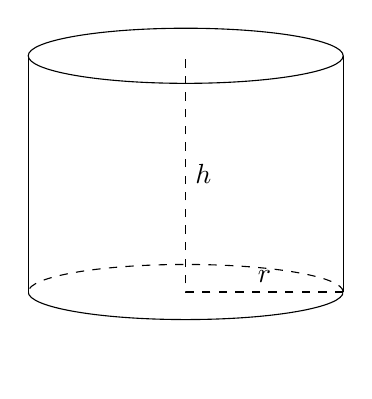
\begin{tikzpicture}
    \begin{scope}
      \clip (-2,0) rectangle (2,1);
      \draw[dashed] (0,0) circle (2 and 0.35);
    \end{scope}
    \begin{scope}
      \clip (-2,0) rectangle (2,-1);
      \draw (0,0) circle (2 and 0.35);
    \end{scope}
    \draw (0,3) circle (2 and 0.35);
    \draw (-2,0) -- (-2,3);
    \draw (2,0) -- (2,3);
    \draw[dashed] (2,0) -- node[above] {\( r \)}
                           coordinate[pos=1](a)(0,0)
                        -- node[right] {\( h \)}
                           coordinate[pos=0.1](b)(0,3);
  \end{tikzpicture}
\end{center}
With the disk method of volume by integration, you can imagine this problem
as an integration problem where a cross section of the cylinder is rotated
an axis. \par
There is another method that uses infinitely small shells which compose the
volume.
\begin{center}
  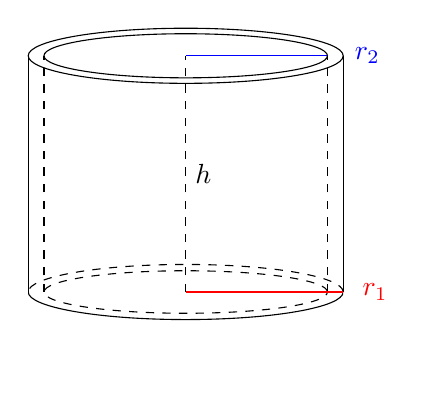
\begin{tikzpicture}
    \begin{scope}
      \clip (-2,0) rectangle (2,1);
      \draw[dashed] (0,0) circle (2 and 0.35);
    \end{scope}
    \begin{scope}
      \clip (-2,0) rectangle (2,-1);
      \draw (0,0) circle (2 and 0.35);
    \end{scope}
    \draw (0,3) circle (2 and 0.35);
    \draw (-2,0) -- (-2,3);
    \draw (2,0) -- (2,3);
    \draw (0,3) circle (1.8 and 0.28);
    \draw[dashed] (-1.8,0) -- (-1.8,3);
    \draw[dashed] (1.8,0) -- (1.8,3);
    \draw[dashed] (0,0) circle (1.8 and 0.27);
    \draw[red] (2,0) -- node[xshift=40] {\( r_{1} \)} coordinate[pos=1](a)(0,0);
    \draw[dashed] (0,0)-- node[right] {\( h \)} coordinate[pos=1](b)(0,3);
    \draw[blue] (0,3) -- node[xshift=40] {\( r_{2} \)}
      coordinate[pos=1](c)(1.8,3);
  \end{tikzpicture}
\end{center}
The volume of the disk is:
\[ V = \pi((r_{1})^{2}-(r_{2})^{2})h \]
\[ V = \lim_{r_{1} \to r_{2}}2\pi\frac{r_{1}+r_{2}}{2}(r_{1}-r_{2})h \]
\[ V = 2\pi\bar{r}(\Delta r)h \]
And as a general form, the sums of the volumes of all the disks that compose
the figure is:
\[ V = \int_{a}^{b}{2\pi xf(x)\diff{x}} \]

\subsection*{Example 1}
\[ y = \frac{1}{x} \quad y = 0 \quad x = 1 \quad x = 2 \]
\begin{center}
  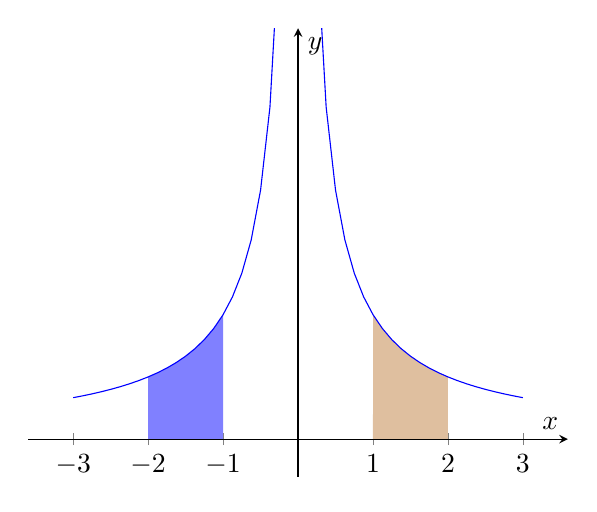
\begin{tikzpicture}
    \begin{axis}[axis lines=middle,
                 xlabel=\(x\),
                 ylabel=\(y\),
                 enlargelimits,
                 ytick=\empty,
                 ymax=3]
    \addplot[name path=F1, blue, domain={0:3}]{1/x};
    \addplot[name path=F2, blue, domain={-3:0}]{-1/x};
    \addplot[name path=G, black, domain={-3:3}]{0};
    \addplot[color=brown!50] fill between [
             of=F1 and G, soft clip={domain=1:2}];
    \addplot[color=blue!50] fill between [
             of=F2 and G, soft clip={domain=-2:-1}];
    \end{axis}
  \end{tikzpicture}
\end{center}
When the red section is rotated about the y-axis, it passes through the
highlighted blue section and the following shape results:
\begin{center}
  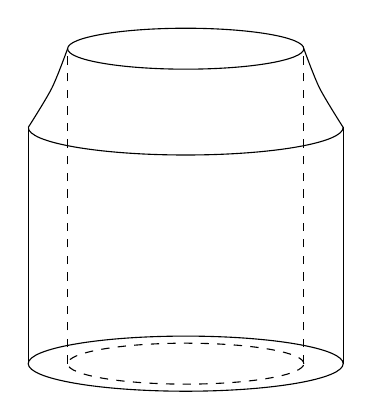
\begin{tikzpicture}
    \draw (0,0) circle (2 and 0.35);
    \begin{scope}
      \clip (-2,3) rectangle (2,2);
      \draw (0,3) circle (2 and 0.35);
    \end{scope}
    \draw (0,4) circle (1.5 and 0.26);
    \draw (-2,0) -- (-2,3);
    \draw (2,0) -- (2,3);
    \draw[dashed] (0,0) circle (1.5 and 0.26);
    \draw[dashed] (-1.5,0) -- (-1.5,4);
    \draw[dashed] (1.5,0) -- (1.5,4);
    \draw plot[smooth] coordinates {(-2,3) (-1.7,3.5) (-1.5,4)};
    \draw plot[smooth] coordinates {(2,3) (1.7,3.5) (1.5,4)};
  \end{tikzpicture}
\end{center}
\[ V = \int_{1}^{2}{2\pi xf(x)\diff{x}} \]
\[ V = 2\pi\int_{1}^{2}{x\frac{1}{x}\diff{x}} \]
\[ V = 2\pi\int_{1}^{2}{\diff{x}} \]
\[ V = 2\pi\bigg[x\bigg]_{1}^{2} \]
\[ V = 2\pi[2-1] = 2\pi \]

\subsection*{Example 2}
\[ y = \e^{-x^{2}} \quad y = 0 \quad x = 0 \quad x = 1 \]
\begin{center}
  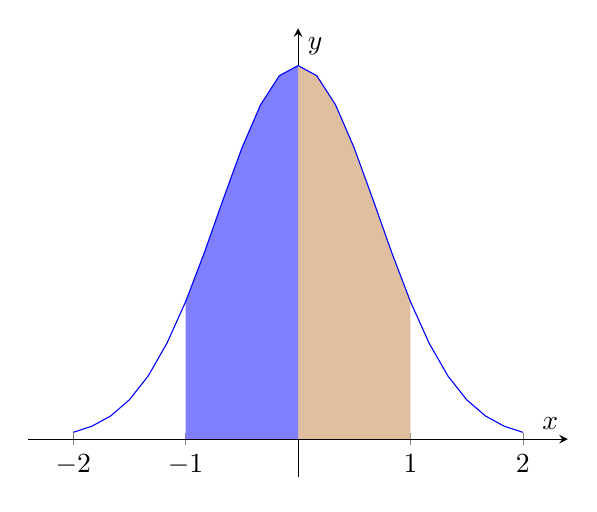
\begin{tikzpicture}
    \begin{axis}[axis lines=middle,
                 xlabel=\(x\),
                 ylabel=\(y\),
                 enlargelimits,
                 ytick=\empty
                ]
    \addplot[name path=F,
             blue,
             domain={-2:2}]{pow(e, -pow(x, 2))};
    \addplot[name path=G,
             black,
             domain={-2:2}]{0};
    \addplot[color=brown!50] fill between [
             of=F and G, soft clip={domain=0:1}];
    \addplot[color=blue!50] fill between [
             of=F and G, soft clip={domain=-1:0}];
    \end{axis}
  \end{tikzpicture}
\end{center}
\[ V = \int_{0}^{1}{2\pi xf(x)\diff{x}} \]
\[ V = \int_{0}^{1}{2\pi x\e^{-x^{2}}\diff{x}} \]
\[ V = -\pi\int_{0}^{1}{-2x\e^{-x^{2}}\diff{x}} \]
\[ V = \pi\bigg[\e^{-x^{2}}\bigg]_{0}^{1} \]
\[ V = \pi\bigg[\e^{0}-\e^{-1}\bigg] \]
\[ V = \pi\bigg[1-\frac{1}{\e}\bigg] \]
\[ V = \pi-\frac{\pi}{\e} \]

\subsection*{Practice Problem 7}
\[ y = 4(x-2)^{2} \quad y = x^{2}-4x+2 \]
\begin{center}
  revolved around the y-axis.
\end{center}
\begin{center}
  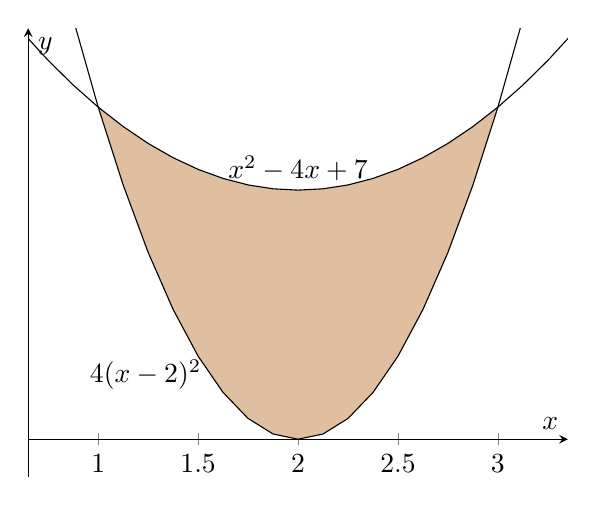
\begin{tikzpicture}
    \begin{axis}[axis lines=middle,
                 xlabel=\(x\),
                 ylabel=\(y\),
                 enlargelimits,
                 ytick=\empty,
                 ymax=4.5
                ]
    \addplot[name path=F, black, domain={0.5:3.5}]{4*(x-2)^2}
        node[pos=0.45, left]{\( 4(x-2)^{2} \)};
    \addplot[name path=G, black, domain={0.5:3.5}]{x^2-4*x+7}
        node[pos=0.5, above]{\( x^{2}-4x+7 \)};
    \addplot[color=brown!50] fill between [
             of=F and G, soft clip={domain=1:3}];
    \end{axis}
  \end{tikzpicture}
\end{center}
\[ V = 2\pi\int_{1}^{3}{x\bigg[(x^{2}-4x+7)+(4(x-2)^{2})\bigg]\diff{x}} \]
\[ V = 2\pi\int_{1}^{3}{x\bigg[x^{3}-4x+7-4x^{2}-16+16x\bigg]\diff{x}} \]
\[ V = 2\pi\int_{1}^{3}{-3x^{3}+12x^{2}-9x\diff{x}} \]
\[ V = 2\pi\bigg[\frac{-3x^{4}}{4}+\frac{12x^{3}}{3}-
    \frac{9x^{2}}{2}\bigg]_{1}^{3} \]
\[ V = 16\pi \]

\begin{center}
  If any errors are found, please contact me at alvin.lin.dev@gmail.com
\end{center}

\end{document}
